\documentclass[12pt,a4paper,bibliography=totoc]{scrreprt}
\usepackage[utf8]{inputenc}
\usepackage[german]{babel}
\usepackage[T1]{fontenc}
\usepackage{amsmath}
\usepackage{amsfonts}
\usepackage{amssymb}
\usepackage{graphicx}
\usepackage{fancyhdr}
\usepackage{placeins}
\usepackage{subfig}
\usepackage[table]{xcolor}
\usepackage{marginnote}
\usepackage{chngcntr}
\usepackage{acronym}
\usepackage{setspace}
\usepackage{enumitem}
\usepackage{notoccite}
\usepackage{siunitx}



\usepackage[scaled]{uarial} % Arial
\renewcommand*{\familydefault}{\sfdefault} %Alles auf Arial



\counterwithout{footnote}{chapter}


\bibliographystyle{unsrt}



%Begin Zeilenabstandskacke

\makeatletter
\newcommand{\MSonehalfspacing}{%
  \setstretch{1.44}%  default
 \ifcase \@ptsize \relax % 10pt
    \setstretch {1.448}%
  \or % 11pt
    \setstretch {1.399}%
  \or % 12pt
   \setstretch {1.433}%
 \fi
}
\newcommand{\MSdoublespacing}{%
  \setstretch {1.92}%  default
  \ifcase \@ptsize \relax % 10pt
    \setstretch {1.936}%
  \or % 11pt
    \setstretch {1.866}%
  \or % 12pt
    \setstretch {1.902}%
  \fi
}
\makeatother
\MSonehalfspacing

%Ende Zeilenabstandskacke


\author{Paula Krenkel}
\title{Steckbrief vom Tabonamitapir}

\date{\today}

\sloppy

\pagestyle{fancy}

\lhead{\begin{small}\slshape  \rightmark \end{small}}
\chead{}
\rhead{\begin{small} \slshape \leftmark \end{small}}

\lfoot{}
\cfoot{\thepage}
\rfoot{}






\begin{document}
\maketitle


\tableofcontents  \thispagestyle{plain}


\cleardoublepage
% \phantomsection
\addcontentsline{toc}{chapter}{\listfigurename} % List of figures in TOC
\listoffigures \thispagestyle{plain}


\cleardoublepage
% \phantomsection
\addcontentsline{toc}{chapter}{\listtablename} % List of tables in TOC
\listoftables


\chapter{Beschreibung}
Der Kabonami-Tapir ist die neuste entdeckte Form der Tapirarten. Ebenfalls ist es das größte neuentdeckte Säugetier seit 100 Jahren und es wurde 08.08.014 gefunden. Insgesamt gibt es 5 verschiedene Arten, wovon der Schabracken Tapir, markant durch sein Schwarz-Weißes Fell, am bekanntesten ist. 

\section{Tabelle}

\begin{table}[h]
\centering
\caption{Tapirarten}
\label{tapirtabl}
\rowcolors{1}{white}{lightgray}
\begin{tabular}{|p{3.5cm}|p{3.5cm}|p{2.5cm}|p{3.5cm}|}
\hline
Art  		 				 & Lateinischer Name  & Vorkommen     & KopfRumpf-Länge in cm 	  	 \\ \hline
Kabomani-Tapir         	  	& Tapirus Kabomani   & Südamerika    & 130          				    \\ \hline
Schabrackentapir        	 & Tapirus indicus    & Asien         & 250-300  						\\ \hline
Bergtapir                	& Tapirus pinchaque  & Südamerika    & 180          					\\ \hline
Flachlandtapir           	& Tapirus terrestris & Südamerika    & 205 (Männchen)  220 (Weibchen) 	\\ \hline	Mittelamerikanischer Tapir 	& Tapirus bairdii    & Mittelamerika & 200 								\\ \hline
\end{tabular}
\end{table} \FloatBarrier



\section{Aussehen}
Äußerlich ähneln Tapire dem Schwein, sind aber genetisch Verwandt mit dem Pferd und dem Nashorn. Sie können eine Körperlänge von circa 100 bis 250 cm erreichen, wobei der Konami-Tapir der Konami-Tapir mit einer ausgewachsenen Körperlänge von circa 130 cm eher zu der kleineren Form gehört. Bis zu 130 Kg kann das Tier werden, was leicht im Gegensatz zu seinen Artgenossen ist, denn diese können ein Gewicht von bis zu 320 Kg erreichen. Man geht auch davon aus, dass bei der Gattung das Weibchen größer als das Männchen ist. Auch das Fell ist  sehr borstig und dunkler, als bei den anderen vier Arten. 
Der Tapir ist durch seinen plumpen, schwerfälligen Körper bekannt, welcher nach hinten hin abgerundet ist und sich vorne am Rüssel hin zuspitzt. Der Rüssel ist ebenfalls sehr charakteristisch für Tapire, denn er dient gleichzeitig auch als Oberlippe. Sie haben kleine ovalförmige Ohren und kleine kurze Beine und sie gehören zu der Gattung der Unpaarhufer \cite{1}. 




\section{Lebensweise}
Tapire sind von Grund auf Einzelgänger und sie verhalten sich aggressiv bei der Begegnung einer Ihrer Artgenossen. Ausgenommen bei der Paarungszeit. Der Kabomani-Tapir ist die kleinste Form der fünf uns heute bekannten Tapire. Neben ihn gibt es noch der Schabrackentapir, den Flachland- und den Bergtapir sowie den Mittelamerikanischen Tapir. Tapire verteidigen ihr Territorium, welches meist zwischen 1 und 8 km$^{2}$ groß ist. Ebenfalls sind Tapire Nachtaktiv, das bedeutet Tagsüber ziehen sie sich ins Unterholz zurück und bei Nachtanbruch gehen sie auf Nahrungssuche. Tapire sind Pflanzenfresser und bevorzugen weiche Nahrung. Ebenfalls leben sie gehäuft in der Nähe von Gewässern. Sie sind sehr gute Schwimmer und Taucher, weswegen sie sich in solchen Gebieten sehr wohl fühlen. Ein Tapir ist auch ein sehr scheues Tier, welches sich bei Gefahr entweder die Flucht zum Wasser ergreifen oder im Zweifelsfall bei einem Angriff beißen. Die natürlichen Feinde eines Tapirs sind größere Raubkatzen, aber auch, je nach Lebensraum auch Bären oder Krokodile. Jedoch ist die größte Gefahr für alle Tapire auf der Welt der Mensch, da er Lebensräume zerstört und auch früher das Fell des Tapirs (speziell das des Schbrackentapirs) sehr begehrt auf dem Markt war.
Über den Kabomani-Tapir ist bisweilen noch nicht allzu viel bekannt, da es sich erst um eine vor nicht allzu langer Zeit entdeckte Rasse handelt. Jedoch geht man davon aus, das ihre Lebensweise der der anderen ähnelt \cite{2}. 


\chapter{Bestand}

\section{Fortpflanzung}
Ein Tapir hat eine Tragezeit der Jungen zwischen 13 und 14 Monate (das entspricht rund 390 bis 410 Tage). Ein Tapir bringt in seinen Leben ein, maximal zwei Jungen zur Welt. Neugeborene ähneln ihrem Fell dem eines Frischlings von Wildschweinen. Ihr Fell ist dunkel, bis hellbraun und ist überzogen mit weißen Streifen, die sich vom Hals über den ganzen Rumpf ziehen. Über die Beine hin gehen die Linien langsam zu Punkten über. Dieses Fell behalten die Jungen ungefähr ihr erstes halbes Lebensjahr bei, bis es dann umschlägt und nach ungefähr einem Jahr haben die Tiere das aussehen eines erwachsenen Tapirs erreicht. Ebenfalls im ersten Lebensjahr bleiben die Jungen noch in der Nähe ihrer Mutter, welche sie in Gefahren beschützt und verteidigt. Nach des ersten Lebensjahres beginnt die Mutter ihr Junges von sich zu entwöhnen. Ab da lebt es als Einzelgänger. Tapire kommen mit den Eintritt ins circa dritte oder vierte Lebensjahr in die Geschlechtsreife und sie  könenn in freier Wildbahn ein Alter von bis zu 30 Jahren erreichen \cite{3}.


\section{Gefährdung/Schutz}
Der Tapir steht unter großer Gefahr. Vor allem, weil es in unserer Welt nur bisweilen fünf bekannte Arten überhaupt gibt. Die mit Abstand größte Gefahr ist die Zerstörung des Lebensraumes der Tapire, da nicht nur ihre Heimat ihnen weggenommen wurde sondern ebenfalls jegliche Rückzugsmöglichkeiten. Die Wälder werden vor allem durch Berbau, Straßenbau,  Industrie und Wohnsiedlungen und natürlich die Vieh- und Landzucht gerodet. Die tropischen Regenwälder haben in den letzten 50 Jahren circa zwei Drittel an Fläche verloren. Ebenfalls sind Tapire durch Krankheiten oft gefährdet, da mit der schon von Beginn an niedrigen Anzahl an Nachkommen und der langen Tragezeit die Fortpflanzungsrate immer weiter sinkt. Eine weitere Gefährdung ist die Jagt von indianischen Völkern, wie zum Beispiel der indigenen Völker in Südamerika auf Tapire. Sie verwenden das Fleisch, da es Proteinhaltig ist und ein Tier eine ganze Familie ernähren kann. Jedoch wurde es auch kommerziell und das Fleisch wurde illegal in Märkten verkauft sowie aus Tapiren produziertes Leder an die Touristen.  
Durch all dies steht zum Beispiel der Bergtapir bei der Naturschutzorganisation IUCN auf der Roten Liste, was eine starke Bedrohung symbolisiert und folglich es ein aussterben in naher Zukunft geben kann. Der Mittelamerimanische Tapir und der Schabrackentapir sind ebenfalls gefährdet und aufgelistet. Nur der Flachlandtapir ist nicht als Bedrohlich eingestuft und ist mit am meisten verbreitet (Stand September 2003). Über den Kabomani Tapir speziell gibt es keinen Eintrag, da die Anzahl an Lebewesen noch nicht bestimmt werden konnte \cite{4}.


\section{Entdeckung}
Die Entdeckung des Kabomanitapirs war so gesehen die größte biologische Entdeckung des 21. Jahrhunderts. Der Wissenschaftler Mario Cozzuol und sein Forscherteam gelang es im Jahr 2013 das Tier im brasilianischen kolumbianischen Grasland und Amazonaswäldern zu entdecken. Jedoch stellte sich für die Wissenschaftler heraus, dass dieses Tier schon entdeckt vorher war. Die in den Gegenden lebenden einheimischen Stämme beschrieben dieses Tier schon lange zuvor und darauf hin entschuldigten sich die Forscher aufrichtig. Die Ureinwohner bezeichnen es, nach der Paumari-Sprache, als ein „Arabo kabomani“, woran als Anerkennung auch der heutige Name, der Kabomanitapir angelehnt ist. 
Obwohl die letzte Tapirart im Jahre 1865 zuletzt gefunden wurde und im Vergleich der vergangenen Jahre mit Abstand das größte Lebewesen seit langem seine Entdeckung macht, ist es dennoch die kleinste lebende Tapirart aktuell. Aber trotz allem zählt der Kabomanitapir mit zu den größten Tieren es südamerikanischen Kontinents \cite{5}. 

\begin{figure}[h]
\begin{center}
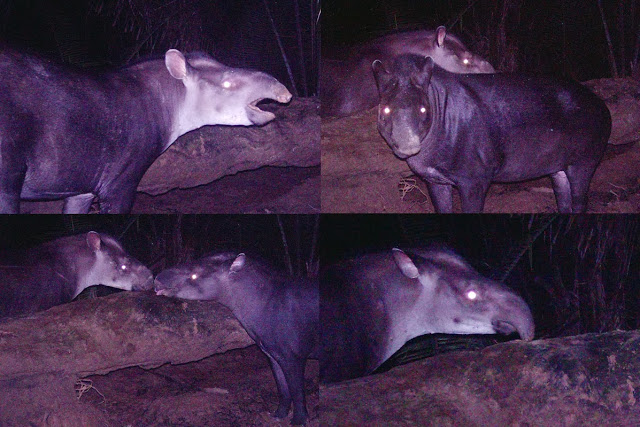
\includegraphics [width=7cm]{kabonami-tapier.jpg}
\caption[Erste Aufnahmen des Kabonamitapirs]{Erste Aufnahmen des Kabonamitapirs}
\label{EKtapir}
\end{center}
\end{figure} \FloatBarrier

\begin{figure}[h]
\begin{center}
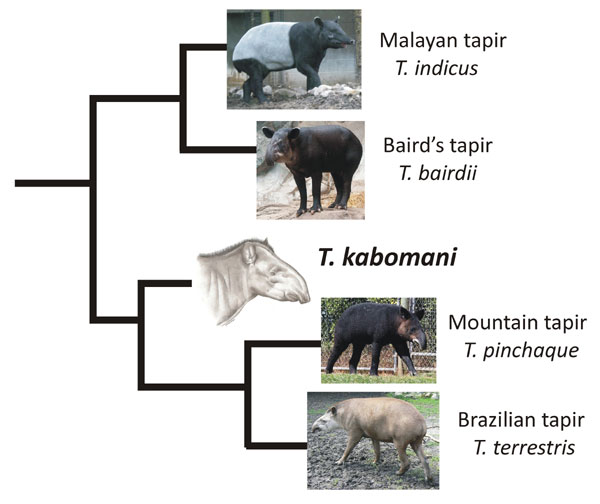
\includegraphics [width=7cm]{Stammbaum.jpg}
\caption[Stammbaum der Tapire]{Stammbaum der Tapire}
\label{Stammtapir}
\end{center}
\end{figure} \FloatBarrier



\clearpage
\pagestyle{plain}
\bibliography{references}




\end{document}
